% ============================================================
%  SCHOLA DOMESTICA — Level 1, Week 2, Lesson 6
%  Topic: Numbers 6 and 7
%  8–10 problems | No speed drill | Picture-heavy
%  Compile with XeLaTeX
%  Place sd_style.sty in curriculum/Level-1/
% ============================================================
\documentclass[12pt,letterpaper]{article}
\usepackage{sd_style}

\renewcommand{\lessonnum}{6}
\renewcommand{\lessonweek}{2}

\begin{document}

\lessonheader{2}{6}{Numbers 6 and 7}

\begin{instructbox}
\noindent\textbf{\color{sd-blue}Instruction} \textit{(read aloud):}\\[4pt]
This week we learn numbers 6 and 7.
Six is one more than five — a whole hand plus one finger.
Seven is one more than six.
Count with me as you point to each picture!
\end{instructbox}

\vspace{8pt}
\noindent\textbf{\color{sd-blue}Trace and write:}
\tracerowpair{6}{7}

\goldrule
\noindent\textbf{\color{sd-blue}Practice}
\vspace{6pt}

\prob Count the dots and write the number.\\[6pt]
\hspace{1cm}\onedot\onedot\onedot\onedot\onedot\onedot\quad\ansblank

\vspace{10pt}
\prob Count the dots and write the number.\\[6pt]
\hspace{1cm}\onedot\onedot\onedot\onedot\onedot\onedot\onedot\quad\ansblank

\vspace{10pt}
\prob How many stars?\\[4pt]
\hspace{1cm}%
\IfFileExists{stars_6.jpg}{
\includegraphics[height=1.4cm]{stars_6.jpg}}{%
  \onestar\onestar\onestar\onestar\onestar\onestar}
\quad\ansblank

\vspace{10pt}
\prob How many?\\[4pt]
\hspace{1cm}%
\IfFileExists{apples_7.jpg}{
\includegraphics[height=1.4cm]{apples_7.jpg}}{%
  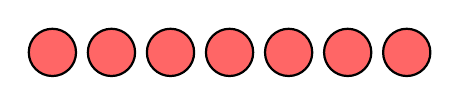
\begin{tikzpicture}[baseline=0]
    \foreach \x in {0,...,6}\draw[fill=red!60,thick](\x*0.75,0)circle(0.3);
  \end{tikzpicture}}
\quad\ansblank

\vspace{10pt}
\prob Circle the correct number.\\[6pt]
\hspace{1cm}%
\IfFileExists{ducks_6.jpg}{
\includegraphics[height=1.4cm]{ducks_6.jpg}}{%
  
\begin{tikzpicture}[baseline=0]
    \foreach \x in {0,...,5}\draw[fill=yellow!70,thick](\x*0.85,0)ellipse(0.32 and 0.22);
  \end{tikzpicture}}
\quad{\Large 5 \quad \textbf{6} \quad 7}

\vspace{10pt}
\prob Draw \textbf{7} circles in the box.\\[4pt]
\noindent\fbox{\rule{0pt}{2.2cm}\hspace{11cm}}

\vspace{10pt}
\prob Write the number that comes after 6: \quad\ansblank

\vspace{10pt}
\prob Write the number that comes before 7: \quad\ansblank

\vspace{10pt}
\prob \textit{(Teacher reads)} There were 5 koi in the pond.
Two more swam in. How many koi are in the pond now?\\[4pt]
\hspace{1cm}\IfFileExists{koi_pond.jpg}{\includegraphics[height=1.6cm]{koi_pond.jpg}}{}
\quad\ansblank

\vspace{10pt}
\prob Put these numbers in order, smallest to largest:\\[4pt]
\hspace{2cm}{\Large 7 \quad 5 \quad 6}
\quad$\longrightarrow$\quad\ansblank\quad\ansblank\quad\ansblank

\goldrule

\begin{checkbox}
\noindent\textbf{\color{sd-green}Knowledge Check}\\[4pt]
\setcounter{probnum}{0}
\prob \onedot\onedot\onedot\onedot\onedot\onedot\onedot\quad How many? \quad\ansblank\\[8pt]
\prob Write the numbers 6 and 7: \quad\ansblank\quad\ansblank
\end{checkbox}

\vfill
\noindent{\color{sd-blue}$\bigstar$ \textbf{Enrichment:}}
In Latin, six is \textit{sex} and seven is \textit{septem}.
Count to seven: \textit{ūnus, duo, trēs, quattuor, quīnque, sex, septem}!

\vspace{4pt}\hrule\vspace{3pt}
{\footnotesize\color{gray}\textit{Teacher note: Use a ten-frame (2×5 grid) to show 6 and 7 as
"five and one more" and "five and two more." This anchors both numbers to 5.}}

\end{document}
